\documentclass[10pt,twocolumn,letterpaper]{article}
\usepackage[final]{cvpr}
\cvprfinalcopy
\usepackage{graphicx}
\usepackage{amsmath}
\usepackage{amssymb}
\usepackage{booktabs}
\usepackage{multirow}
\usepackage{array}
\usepackage{tabularx}
\usepackage{makecell}
\usepackage{enumitem}
\usepackage[pagebackref=false,breaklinks=true,colorlinks=true,citecolor=blue,linkcolor=blue,urlcolor=blue]{hyperref}
\usepackage{tikz}
\usetikzlibrary{arrows.meta,positioning,shapes.geometric,fit}
\usepackage{xspace}

\setlength{\textfloatsep}{8pt plus 1pt minus 2pt}
\setlength{\floatsep}{8pt plus 1pt minus 2pt}
\setlength{\intextsep}{8pt plus 1pt minus 2pt}

\newcommand{\method}{Selective Object-Patch Verification\xspace}
\newcommand{\sr}{\mathrm{SR}}
\newcommand{\spl}{\mathrm{SPL}}
\newcommand{\dtg}{\mathrm{DTG}}
\newcommand{\steps}{\mathrm{Steps}}

\title{From Semantic Frontiers to Selective Vision-Language Verification for Zero-Shot Object Navigation}

\author{AIAA 3201 Project Team\\
The Hong Kong University of Science and Technology (Guangzhou)\\
}

\begin{document}
\maketitle
\thispagestyle{empty}

\begin{abstract}
Zero-shot object-goal navigation asks an embodied agent to find a target category in a previously unseen indoor scene without task-specific training. This project studies the evolution from 2D vision-language semantic priors to LLM-guided navigation and finally to a lightweight vision-language verifier for final target confirmation. We first implement the required Part 1 Plan A dense semantic-map pipeline and the Plan B VLFM-style frontier scorer on HM3D and MP3D. After fixing the Plan A recovery loop and active-goal replanning, the repaired dense-map branch reaches 48.50\% SR / 13.28\% SPL on a 200-episode HM3D subset and 51.00\% SR / 13.69\% SPL on a 200-episode MP3D subset, while VLFM Plan B reaches 52.30\% SR and 30.34\% SPL on HM3D. We then reproduce an ASCENT-style LLM-driven ObjectNav system with RGB-D mapping, frontier exploration, stair heuristics, and semantic value maps; the DeepSeek ASCENT-Single 1000-episode baseline reaches 64.50\% SR and 33.36\% SPL. Finally, selective verification gives a controlled fixed-200 improvement from 130/200 to 132/200 successes by reducing false positives from 36 to 33. Code, logs, and reproduction instructions: \url{https://github.com/Demonmasterlqx/AIAA-3201-Intro2CV-Project}.
\end{abstract}

\section{Introduction}
Object-goal navigation has become a compact testbed for embodied perception, mapping, and high-level reasoning. In zero-shot ObjectNav, the agent receives only a target category, such as \emph{chair} or \emph{toilet}, and must navigate using RGB-D observations in unseen scenes. The setting is appealing for computer vision because success requires both local recognition and spatial decision-making: a visual-language model may recognize semantic cues, but the agent must still choose frontiers, recover from occlusion, and stop only when the object is truly reached.

This project follows the roadmap in the course specification: Part 1 studies 2D semantic priors through ZSON~\cite{zson2022} and VLFM~\cite{vlfm2024}; Part 2 moves to a stronger ASCENT-style LLM-guided pipeline inspired by adaptive and floor-aware navigation systems~\cite{apexnav2025,stairway2026}; Part 3 investigates generative and large-model cognitive enhancement through a Qwen-VL verifier. The central lesson is that stronger recognition is not automatically stronger navigation. A VLM can reduce semantic false positives at the final stop gate, but if invoked too often or too conservatively it increases path length and shifts failures into never-saw-target or false-negative modes.

The project is deliberately framed as a reproduction-and-improvement study rather than a single new architecture trained end-to-end. This matters for zero-shot navigation: the strongest systems are often assemblies of mapping, frontier selection, object proposal, language reasoning, and stop-decision modules. An improvement in one module can disappear if it changes the operating point of another module. For example, a stricter verifier can make fewer incorrect stops while also rejecting marginal true positives, forcing longer exploration and reducing SPL. We therefore report both aggregate metrics and failure buckets.

Figure~\ref{fig:pipeline} summarizes the resulting three-stage system. The final method keeps the efficient ASCENT exploration backbone and uses Qwen-VL selectively, only when BLIP2-based final confirmation is risky or ambiguous. This design mirrors the practical constraint of embodied navigation: compute should be spent on hard semantic decisions, not on every observation.

\begin{figure*}[t]
  \centering
  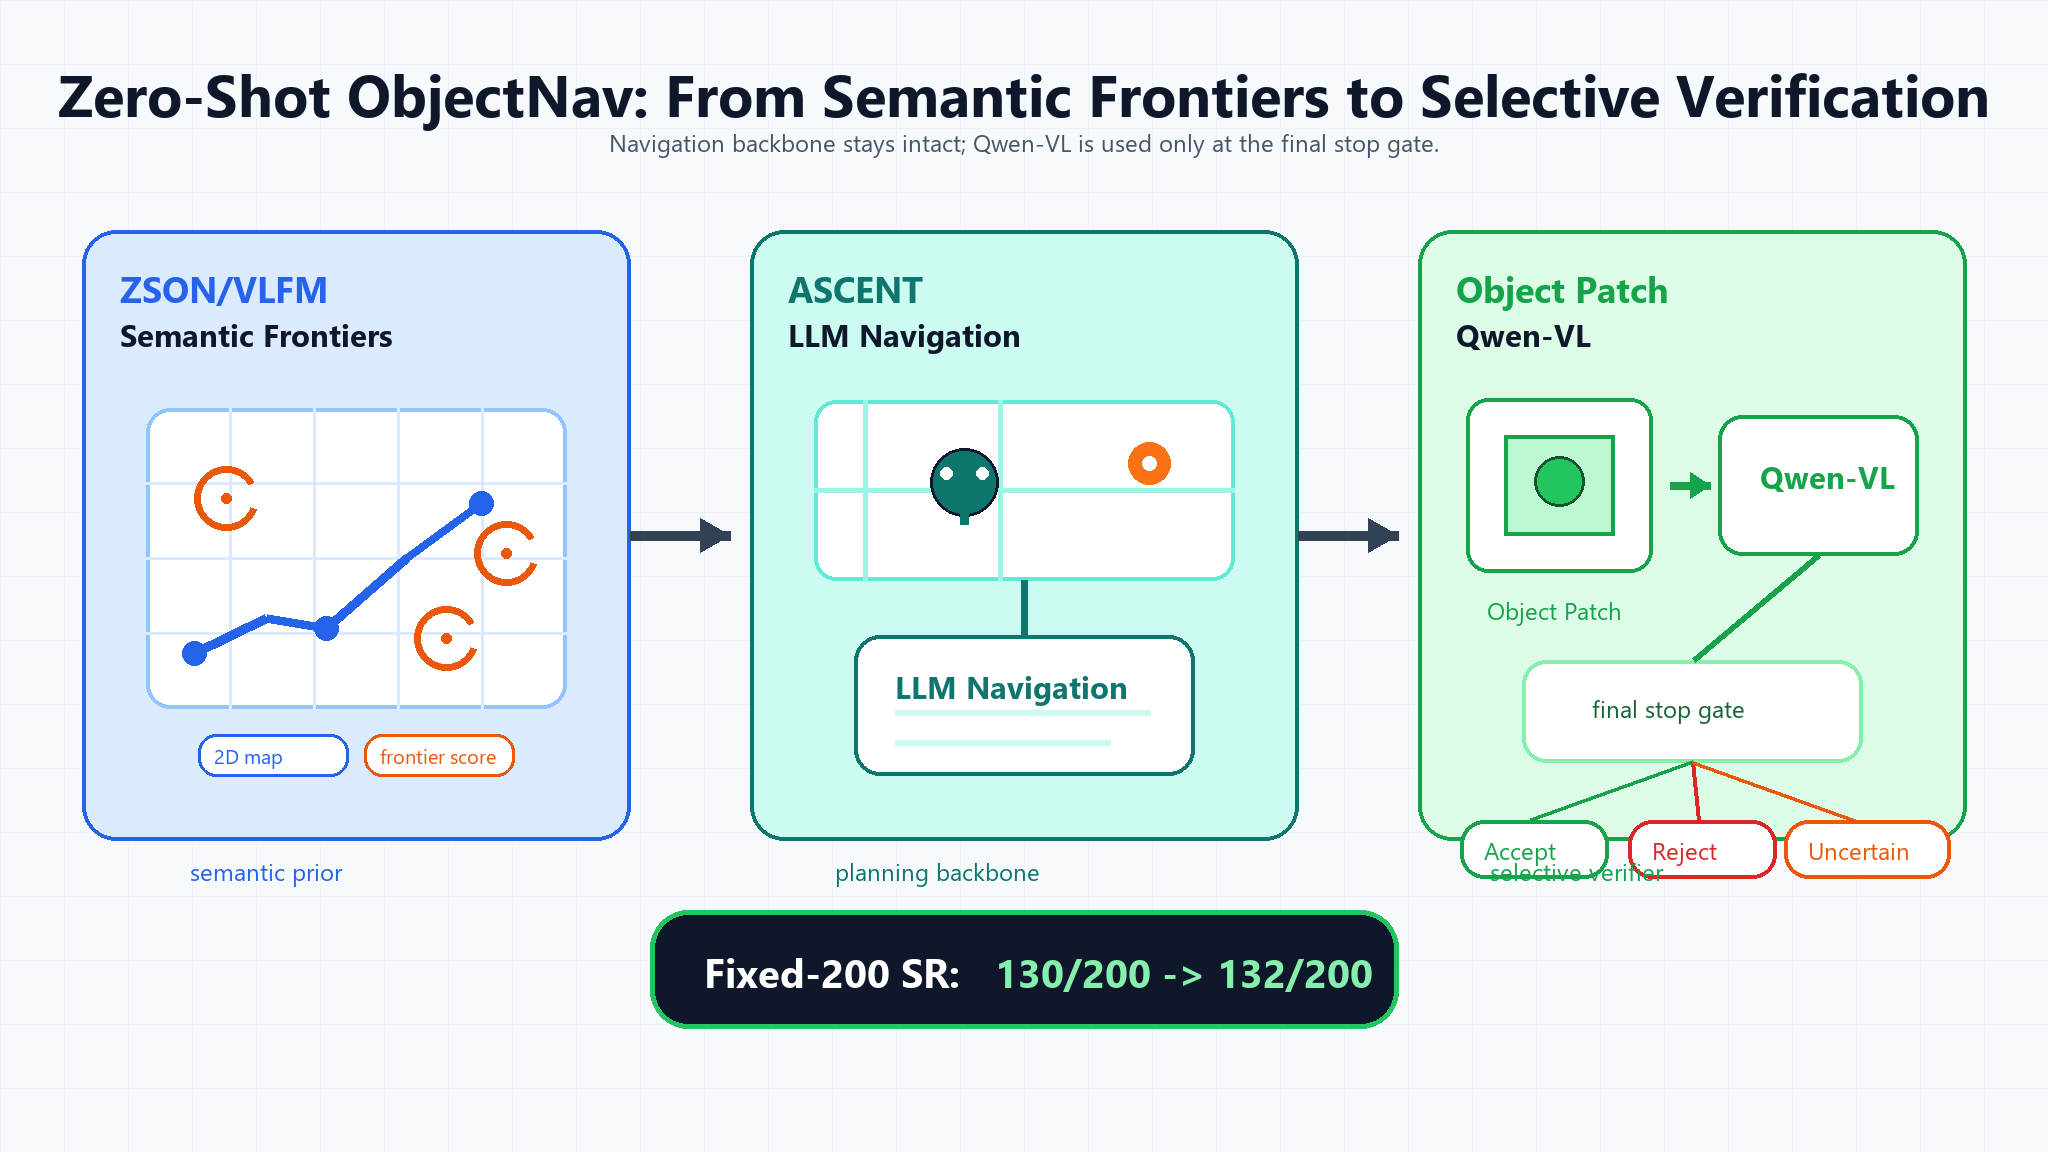
\includegraphics[width=0.95\linewidth]{figures/pipeline_overview_gpt2.png}
  \caption{Project overview. Part 1 evaluates 2D semantic priors with the required Plan A dense semantic-map implementation and VLFM Plan B frontier scoring. Part 2 reproduces an ASCENT-style LLM-driven navigation baseline. Part 3 adds selective Qwen-VL object-patch verification at the final stop gate, routing object crops into accept/reject/uncertain decisions and improving the fixed-200 comparison from 130/200 to 132/200 successes.}
  \label{fig:pipeline}
\end{figure*}

Our contributions are threefold. First, we build a reproducible evaluation record across ZSON, VLFM, and ASCENT-style systems on HM3D/MP3D. Second, we identify false-positive final stops as a stable failure mode across baselines. Third, we show that object-patch VLM verification is most effective as a targeted confidence-fusion module rather than a full replacement for BLIP2-based final checking.

The resulting report is organized around the same evidence chain. Section~2 places the work among zero-shot semantic navigation, embodied benchmarks, LLM navigation, and large vision-language verification. Section~3 describes the three-stage method. Section~4 gives quantitative results, including ablations that failed. Section~5 discusses representative trajectories and failure modes.

\section{Related Work}
\textbf{Zero-shot semantic navigation.} ZSON~\cite{zson2022} introduced multimodal goal embeddings for zero-shot object-goal navigation. CoW~\cite{cow2023} and VLFM~\cite{vlfm2024} further show that CLIP-like or image-text matching models can guide exploration without category-specific training. Our Part 1 includes the required Plan A dense semantic-map implementation and VLFM Plan B.

These methods share an important design philosophy: semantic knowledge is imported from pretrained image-language models rather than learned from ObjectNav reward. This makes them attractive for small projects and for open-vocabulary deployment, but it also exposes a gap between recognition and control. A pretrained matcher can assign high similarity to a view or region without providing a stable reachable goal point. In practice, the navigation wrapper must decide how to aggregate observations, when to revisit a suspected target, and when to stop.

\textbf{Embodied simulators and metrics.} We evaluate in Habitat-Sim~\cite{habitat2019} using HM3D~\cite{hm3d2021} and MP3D~\cite{matterport2017}, two standard indoor navigation datasets. AI2-THOR~\cite{ai2thor2017} and Gibson~\cite{gibson2018} are alternative embodied environments. We report success rate and SPL following the embodied navigation evaluation protocol~\cite{spl2018}.

SR measures whether the agent stops near an instance of the requested category, while SPL discounts successful trajectories that are much longer than the shortest path. We also report DTG and step count where available. These secondary metrics are useful for diagnosing verifier changes: a method may preserve SR while increasing steps, or reduce false positives while raising final distance because it continues exploring after rejecting a candidate.

\textbf{3D memory, adaptive exploration, and LLM planning.} Recent methods add richer spatial memory and reasoning. ConceptGraphs~\cite{conceptgraphs2024} and SG-Nav~\cite{sgnav2024} use open-vocabulary 3D scene graphs to connect perception with planning. MG-Nav~\cite{mgnav2025}, UniGoal~\cite{unigoal2025}, ApexNav~\cite{apexnav2025}, CogNav~\cite{cognav2025}, and Stairway to Success~\cite{stairway2026} explore sparse memory, universal goals, adaptive exploration, cognitive process modeling, and floor-aware search. Multi-agent settings such as PARTNR~\cite{partnr2024} motivate collaborative exploration, but our negative-control experiments show that naive multi-agent rollout can degrade ObjectNav without explicit coordination.

\textbf{Large vision-language verification.} BLIP2~\cite{blip22023} provides a compact image-text matching signal for semantic maps and final target checks. Qwen2.5-VL~\cite{qwen25vl2025} can perform richer visual reasoning, but whole-frame verification is noisy under clutter. We therefore segment detector proposals using MobileSAM~\cite{mobilesam2023} and ask Qwen-VL about local object patches, turning VLM reasoning into a confidence-fusion module.

\begin{table*}[t]
\centering
\small
\caption{Main controlled comparison on the fixed-200 subset. The selective hybrid improves the final stop decision while keeping the ASCENT exploration backbone; bold numbers mark metrics where our method is better than the matched baseline.}
\label{tab:main}
\begin{tabular}{lrrrrrrr}
\toprule
Method & Successes & SR (\%) & SPL (\%) & False pos. $\downarrow$ & Failures $\downarrow$ & DTG & Steps \\
\midrule
Fixed-200 Local-Qwen baseline & 130/200 & 65.00 & 35.09 & 36 & 70 & 3.044 & 180.00 \\
Fixed-200 DeepSeek selective hybrid (ours) & \textbf{132/200} & \textbf{66.00} & \textbf{35.19} & \textbf{33} & \textbf{68} & 3.114 & 183.79 \\
\bottomrule
\end{tabular}
\end{table*}

\section{Method}
\subsection{Problem Formulation}
An episode is specified by a previously unseen scene, an initial pose, and a target object category. At each step the agent observes RGB-D input and must choose a navigation action or a final stop action. A run is successful if the stop action occurs within the benchmark success radius of a visible or reachable target instance. We denote success rate by $\sr$ and SPL by $\spl$. We use the same simulator-level episode definitions for baseline and variant comparisons whenever the result is used as a positive claim.

The project contains three increasingly strong policy families. The first family creates 2D semantic maps from vision-language features. The second family reproduces ASCENT-style LLM-guided search with semantic memory. The third family keeps the ASCENT search policy but changes the final target verification rule. The design goal for Part 3 is narrow: reduce wrong stops on distractor objects without damaging the exploration behavior that made ASCENT strong.

\subsection{Part 1: 2D Semantic Priors}
Plan A is our required dense semantic-map implementation. It uses frozen CLIP patch features, depth, pose, and Habitat top-down maps to project goal-conditioned similarity into a 2D map. A heuristic planner then chooses either high-similarity semantic cells or unexplored frontiers and uses a shortest-path follower to move toward the selected subgoal.

The VLFM-style baseline instead scores unexplored frontiers using the current RGB observation and a vision-language image-text matching model. Frontier restriction makes exploration less dense and more goal-directed: rather than searching all mapped pixels, the agent selects frontiers with high semantic promise and switches to point navigation once a target point cloud is confirmed.

Concretely, the dense-map variant treats each projected map cell as a potential semantic memory slot. A score map is produced by comparing stored visual features with a text embedding of the goal category, and the planner chooses reachable high-score cells. The failure mode is that a high score may correspond to a transient view, projection noise, or a semantically related distractor. The frontier variant changes the action space from ``go to the best semantic pixel'' to ``inspect the most promising unexplored boundary.'' This reduces the demand on long-horizon feature stability and better matches embodied exploration.

\subsection{Part 1 Reproduction Choices}
The Part 1 goal is not to tune a new model but to implement the requested reproduction branches and identify which ones work. We therefore report Plan A directly as our hand-built dense-map branch. The initial full-val implementation exposed a control bug: stuck recovery repeatedly reset the same action queue, so many episodes never returned to meaningful replanning. After repairing the recovery state machine and active-goal selection, we rerun 200-episode HM3D/MP3D subsets and report those fixed Plan A results. VLFM Plan B remains the strongest completed Part 1 artifact with full-val HM3D evidence.

\subsection{Part 2: ASCENT-Style LLM Navigation}
For the SOTA reproduction stage, we use an ASCENT-style pipeline combining RGB-D mapping, object detection, a semantic value map, frontier exploration, stair/floor heuristics, and a high-level LLM planner. The planner reasons over target category, frontier descriptions, room priors, and floor cues. The baseline final-check module uses BLIP2 cosine double-checking near suspected targets. We treat the DeepSeek ASCENT-Single 1000-episode run as the main full-scale Part 2 baseline.

We also evaluate a naive two-agent variant as a negative control. It launches multiple embodied agents but lacks mature role assignment, frontier ownership, communication, or target fusion. This is useful because it separates genuine cognitive improvement from simply adding more moving parts.

The ASCENT-style loop maintains two coupled memories. The geometric map tracks explored free space, obstacles, and frontiers. The semantic memory stores object detections and language-derived target priors. At decision time, the LLM planner does not directly control low-level motion; instead it biases the choice of frontier or local search region. This separation is important because low-level PointNav and collision recovery remain deterministic and fast, while the LLM is used only for high-level reasoning over a compact state description.

The baseline stopping rule is intentionally lightweight. Once the planner believes the target is nearby, BLIP2 compares the goal text against the current visual evidence and a small set of candidate views. This makes final checking cheap enough to run frequently, but it is susceptible to visually or contextually related distractors. Examples include accepting a couch when the target is a bed-like object, accepting a screen-like region for TV-related goals, or accepting clutter with the correct room context but no true object instance.

\subsection{Part 3: Selective Object-Patch Verification}
The Part 3 enhancement targets false-positive stops. When ASCENT approaches a suspected target, object detections provide bounding boxes. We crop and mask the candidate object with MobileSAM and ask Qwen-VL a constrained question: whether the patch contains the requested category and how confident the decision is. Object patches reduce background and room-context distractions compared with full-frame VLM verification.

However, replacing every final check with Qwen-VL is expensive and overly conservative. The final system is therefore selective: BLIP2 remains the default, while Qwen-VL is triggered for high-risk or boundary cases. The verifier returns a tri-state decision, \emph{accept}, \emph{reject}, or \emph{uncertain}; uncertain cases permit additional local observation rather than immediate abandonment. For TV/screen-like ambiguity, a high-confidence BLIP fallback prevents over-rejection. Figure~\ref{fig:qual_part3} shows the same fixed demonstration case where the baseline false-positively stops, while the selective verifier continues and succeeds.

The selective gate uses three practical signals: the baseline BLIP2 confidence, category-specific ambiguity, and whether the object proposal is spatially consistent with the mapped target point. If BLIP2 is strongly positive on an easy category, the system accepts without calling Qwen-VL. If the score lies near a decision boundary, or if the category is known to create distractors, the object-patch verifier is called. If Qwen-VL rejects the proposal, the stop action is suppressed and the location is marked as a rejected candidate so that the agent continues exploration instead of immediately reconsidering the same view. The resulting operating statistics are reported with the ablations in Table~\ref{tab:diagnostics}.

\section{Experiments}
\subsection{Setup}
All navigation experiments use Habitat-style ObjectNav episodes in HM3D and MP3D. We report SR, SPL, final distance-to-goal (DTG) when available, and average steps. Small 8/20-episode runs are used for ablations and diagnostics; 100-episode and 200-episode fixed subsets are used for controlled comparisons; 1000-episode runs are used for scale checks. Qualitative figures are extracted from selected run videos and semantic-map snapshots.

The submitted results folder is intentionally small. Instead of duplicating full scene datasets, model checkpoints, or multi-gigabyte debug folders, we keep run logs, summary JSON/CSV files, selected videos, and selected still frames. This makes the report reproducible at the level of reported metrics and qualitative examples while avoiding raw data duplication. The final positive comparison uses a fixed 200-episode subset so that the Local-Qwen baseline and DeepSeek selective hybrid see the same episodes.

\begin{table*}[t]
\centering
\footnotesize
\caption{Part 1 reproduction results. Plan A is the required dense semantic-map implementation; the rows below use the repaired active-goal controller on 200-episode subsets. The Plan A subset runs use an evaluation success-radius stop gate, discussed in Sec.~\ref{sec:quantitative}.}
\label{tab:part1}
\begin{tabular}{@{}llrrrr@{}}
\toprule
Method & Dataset & Episodes & SR (\%) & SPL (\%) & Avg. steps \\
\midrule
ZSON Plan A active-goal & HM3D val & 200/200 & 48.50 & 13.28 & 377.43 \\
ZSON Plan A active-goal & MP3D val & 200/200 & 51.00 & 13.69 & 359.53 \\
VLFM Plan B & HM3D val & 2000/2000 & 52.30 & 30.34 & 156.11 \\
VLFM Plan B & MP3D val & 1310/2195 & 26.18 & 12.58 & 246.40 \\
\bottomrule
\end{tabular}
\end{table*}

\begin{table*}[t]
\centering
\small
\caption{ASCENT and Qwen-VL verifier experiments. The full object-patch verifier improves the matched 20-episode subset but does not beat the full 1000-episode ASCENT baseline; the fixed-200 final comparison is separated in Table~\ref{tab:main}.}
\label{tab:ascent}
\begin{tabular}{llrrrr}
\toprule
Experiment & Sample & SR (\%) & SPL (\%) & DTG & Steps \\
\midrule
ASCENT-Single baseline & 20 ep & 80.00 & 43.50 & 1.675 & 142.10 \\
ASCENT-2Agents-Naive & 20 ep & 45.00 & 5.46 & 1.213 & 164.25 \\
Qwen-VL full-frame & 20 ep & 65.00 & 29.74 & 3.424 & 248.60 \\
Qwen-VL object-patch weakcache & 20 ep & 85.00 & 36.62 & 1.794 & 240.95 \\
ASCENT-Single DeepSeek & 1000 ep & 64.50 & 33.36 & 2.793 & 187.98 \\
Qwen object-patch v4 & 1000 ep & 61.40 & 30.26 & 2.893 & 233.67 \\
Local-Qwen selective hybrid & 1000 ep & 64.10 & 32.19 & 2.890 & 193.39 \\
\bottomrule
\end{tabular}
\end{table*}

\begin{table*}[t]
\centering
\footnotesize
\caption{Compact diagnostic tables for selective verification. Left: failure buckets show that the fixed-200 gain mainly comes from fewer false-positive stops. Right: operating statistics show that Qwen-VL is used as a targeted verifier rather than a universal replacement for BLIP2.}
\label{tab:diagnostics}
\begin{minipage}[t]{0.48\linewidth}
\centering
\begin{tabular}{lrrr}
\toprule
Run & False pos. & Never-saw & Failures \\
\midrule
Local-Qwen 100 baseline & 44 & 15 & 59 \\
Local-Qwen 100 selective & 39 & 18 & 57 \\
Fixed-200 baseline & 36 & 34 & 70 \\
Fixed-200 selective & 33 & 35 & 68 \\
\bottomrule
\end{tabular}
\end{minipage}
\hfill
\begin{minipage}[t]{0.48\linewidth}
\centering
\begin{tabular}{lrr}
\toprule
Statistic & 1000 ep & Fixed-200 \\
\midrule
BLIP2 default checks & 3771 & 618 \\
Qwen object-patch checks & 1343 & 232 \\
Boundary-gate cases & 488 & 102 \\
Verifier accepts & 791 & 163 \\
Verifier rejects & 4406 & 725 \\
Verifier uncertain & 405 & 64 \\
\bottomrule
\end{tabular}
\end{minipage}
\end{table*}

\subsection{Quantitative Findings}
\label{sec:quantitative}
Table~\ref{tab:main} is the primary result used for the final positive claim. On the same fixed-200 subset, selective hybrid verification improves from 130/200 to 132/200 successes, with SR rising from 65.00\% to 66.00\% and SPL rising from 35.09\% to 35.19\%. The improvement comes from fewer false-positive stops: 36 in the baseline and 33 in our final method.

Table~\ref{tab:part1} reports the required Plan A branch directly using the repaired active-goal controller. The original full-val diagnostic run reached near-zero SR because recovery restarted every step and repeatedly executed the first recovery action instead of returning to semantic/frontier replanning. After fixing this state machine and rerunning 200-episode subsets, Plan A reaches 48.50\% SR / 13.28\% SPL on HM3D and 51.00\% SR / 13.69\% SPL on MP3D. These runs use an evaluation success-radius stop gate, so we treat them as repaired Plan A subset evidence rather than a strict non-oracle full benchmark. VLFM Plan B remains the strongest completed full-val Part 1 baseline in our runs: on HM3D it reaches higher SR and SPL while using fewer average steps than repaired Plan A, showing the exploration-efficiency advantage of frontier scoring over dense-map goal chasing.

Table~\ref{tab:ascent} shows that ASCENT-Single is a strong Part 2 baseline. Naive multi-agent exploration is not a free improvement: SR drops from 80\% to 45\% on the matched small subset. Full-frame Qwen-VL also underperforms, indicating that VLM capacity alone does not solve final target ambiguity. Object-patch verification is better: it reaches 85\% SR on 20 episodes and removes false-positive failures in that subset. At 1000 episodes, however, full object-patch verification remains below the ASCENT baseline because conservative verification increases steps and transfers errors into false negatives or never-saw failures.

The final fixed-200 comparison is therefore intentionally modest but controlled. As Table~\ref{tab:diagnostics} shows, the same trend appears in the failure buckets: selective verification reduces false-positive stops while slightly increasing never-saw outcomes. The operating counts also explain why this does not become a full replacement strategy: Qwen-VL is invoked only for a targeted subset of ambiguous or risky checks.

\subsection{Why Some Variants Are Not Final}
Several implemented variants are useful evidence but should not be presented as the final improvement. The multi-agent ASCENT branch is a negative control: without coordination and map sharing, multiple agents create duplicated exploration and inconsistent stop decisions. The Qwen-VL full-frame branch tests a tempting shortcut, but whole-frame prompts are vulnerable to background semantics and room priors. The object-patch weakcache branch is important because it demonstrates that local visual verification can remove false positives on a small subset; however, its 1000-episode rerun does not beat the DeepSeek ASCENT baseline.

The final claim is therefore narrower: selective object-patch verification gives the cleanest fixed-subset improvement. This is also the most scientifically defensible claim because it compares two methods on the same 200 episodes and explains the gain through a measured change in failure buckets.

\subsection{Failure Taxonomy}
We divide failed episodes into three coarse buckets. A \emph{false positive} means the agent stopped near an incorrect object or distractor. A \emph{never-saw} failure means the agent did not obtain useful target evidence before timeout or termination. A \emph{false negative} or over-rejection case means a plausible target was observed but the verifier did not accept it. The tables aggregate false negatives into the remaining failures when the logs do not expose a separate stable label.

The selective verifier directly targets only the first bucket. This explains both the success and the limitation of Part 3. On fixed-200, false positives fall from 36 to 33, producing two additional successes. At the same time, never-saw failures rise slightly from 34 to 35 because rejected candidates can consume extra steps and push the agent into longer exploration. The method is therefore best viewed as changing the stop-decision operating point rather than solving exploration.

Table~\ref{tab:diagnostics} shows the intended operating regime. The system still performs many cheap BLIP2 checks, but routes a smaller subset of semantically risky cases to Qwen-VL. The large number of rejections is expected because most explored observations do not contain the target. The useful behavior is not merely rejecting more; it is rejecting the right final-stop candidates while leaving confident true positives untouched.

\section{Qualitative Analysis}
\begin{figure}[t]
  \centering
  \begin{tabular}{@{}cc@{}}
    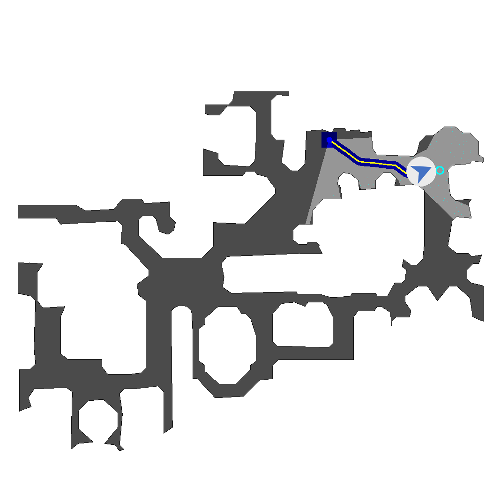
\includegraphics[width=0.45\linewidth]{figures/zson_semantic_success.png} &
    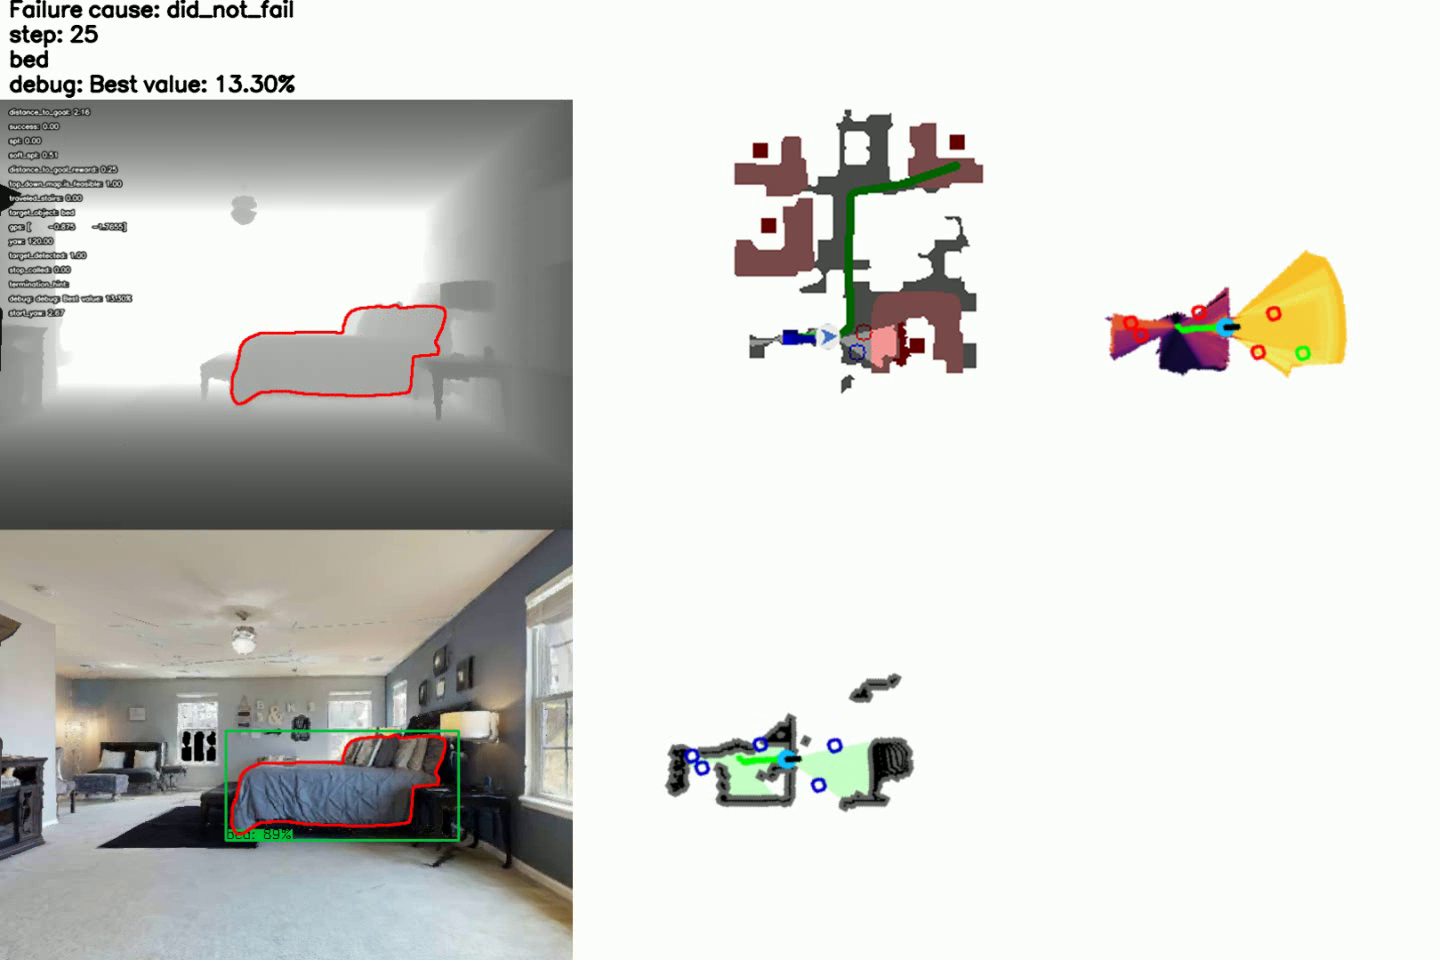
\includegraphics[width=0.45\linewidth]{figures/vlfm_hm3d_success_frame.png} \\
    \small ZSON semantic map & \small VLFM trajectory frame \\
    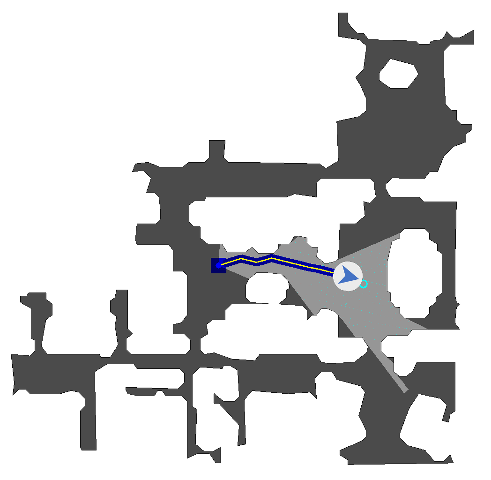
\includegraphics[width=0.45\linewidth]{figures/zson_semantic_failure.png} &
    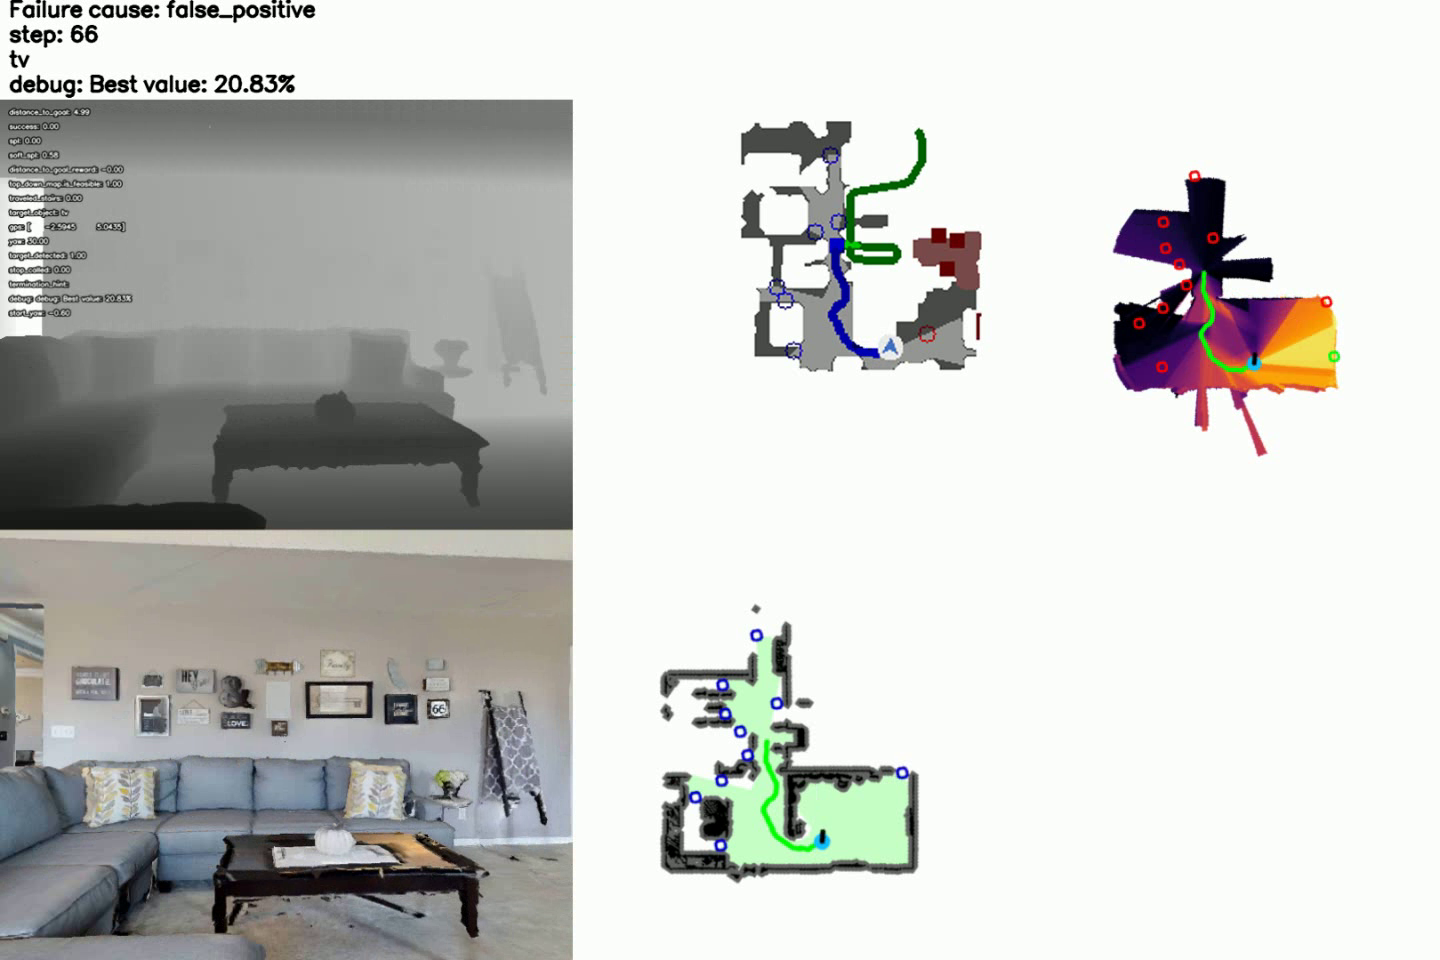
\includegraphics[width=0.45\linewidth]{figures/vlfm_hm3d_failure_frame.png} \\
    \small Diagnostic failure map & \small Plan B failure frame
  \end{tabular}
  \caption{Part 1 qualitative examples. The required Plan A dense-map branch provides useful visual evidence, and the repaired active-goal controller turns this into nontrivial subset performance. Frontier-based VLFM trajectories remain more behaviorally stable, yet still fail under ambiguous or occluded targets.}
  \label{fig:qual_part1}
\end{figure}

\begin{figure}[t]
  \centering
  \begin{tabular}{@{}cc@{}}
    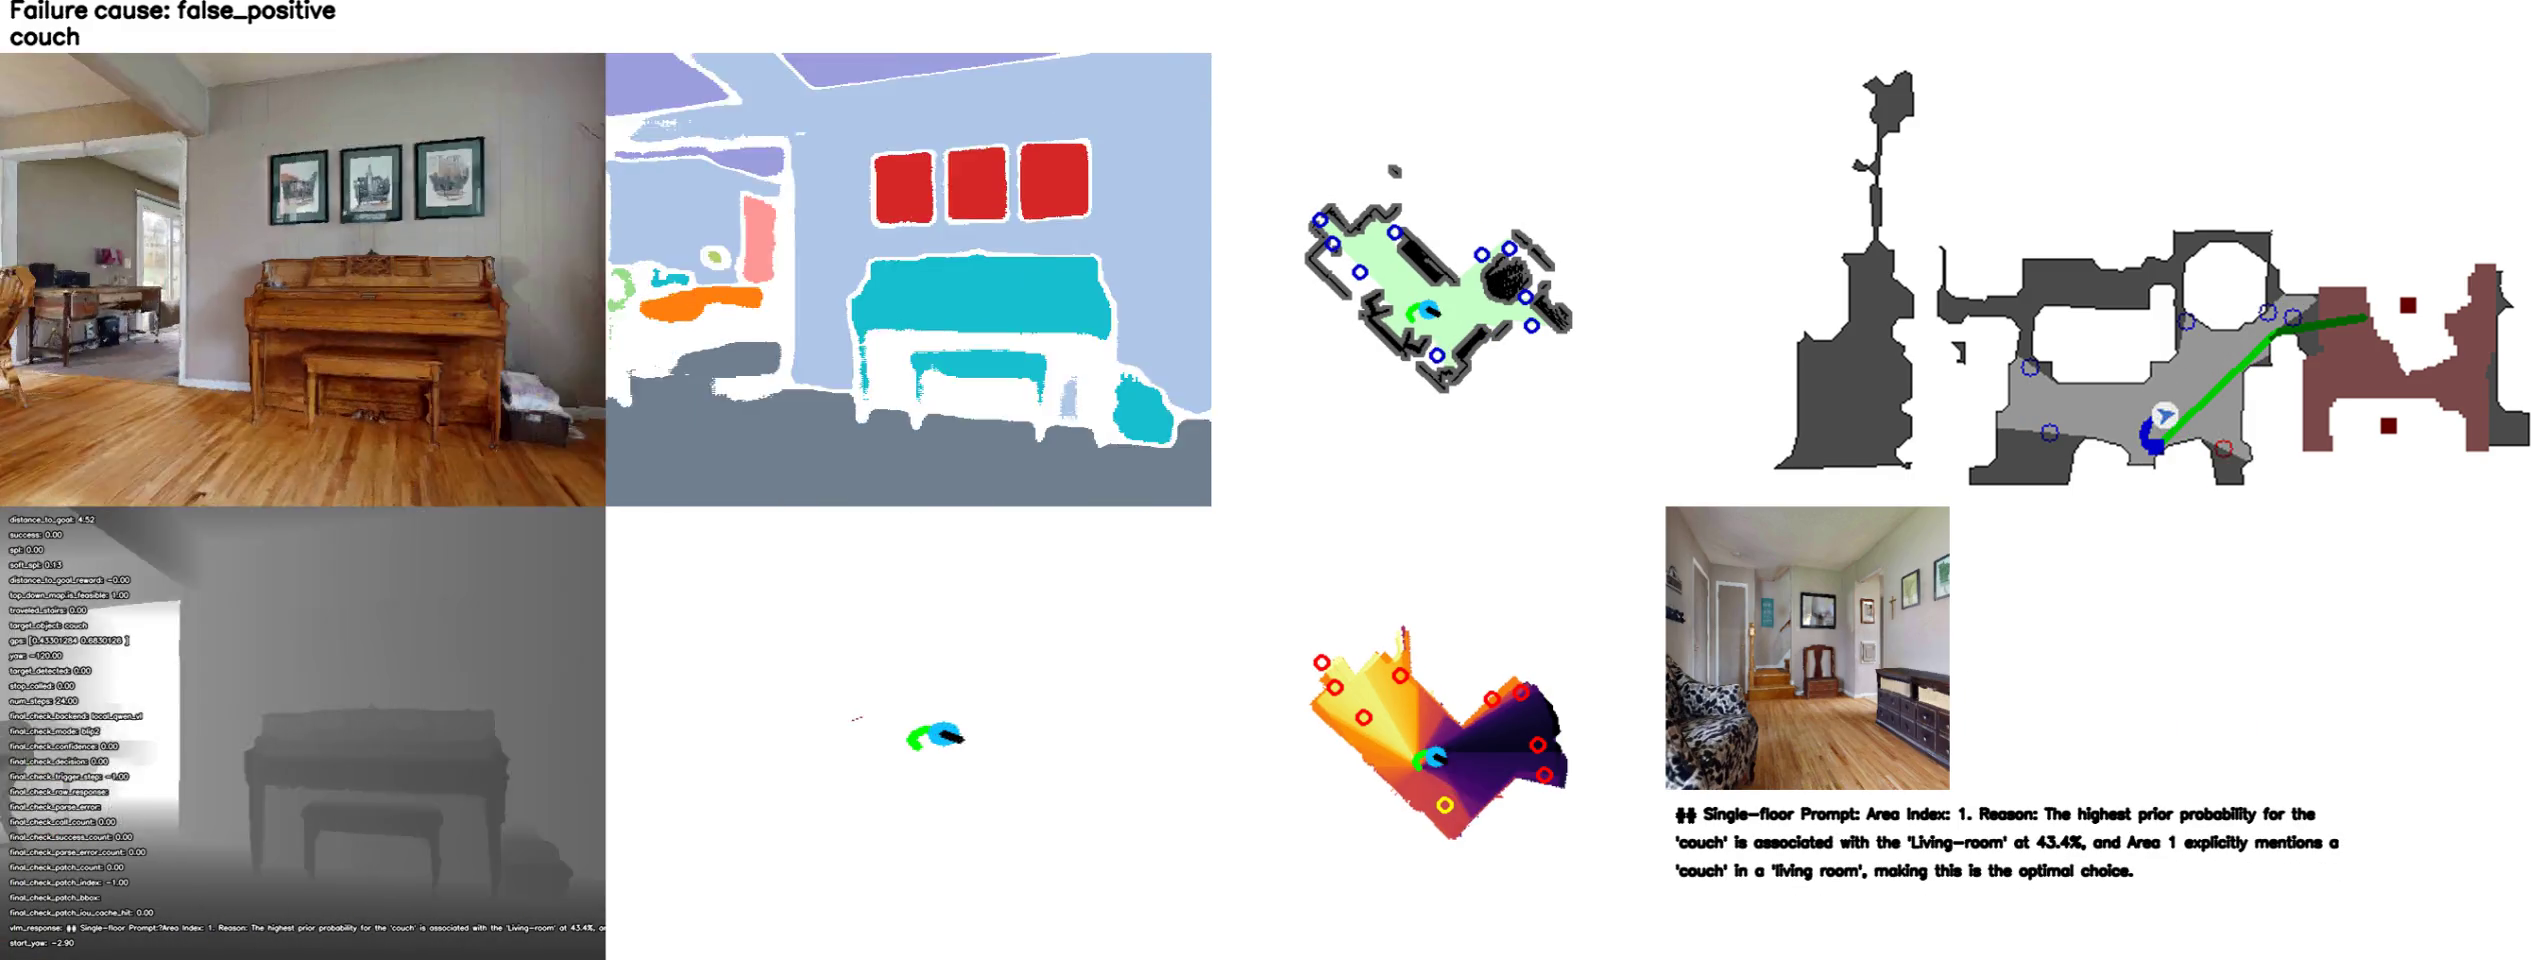
\includegraphics[width=0.45\linewidth]{figures/ascent_baseline_false_positive.png} &
    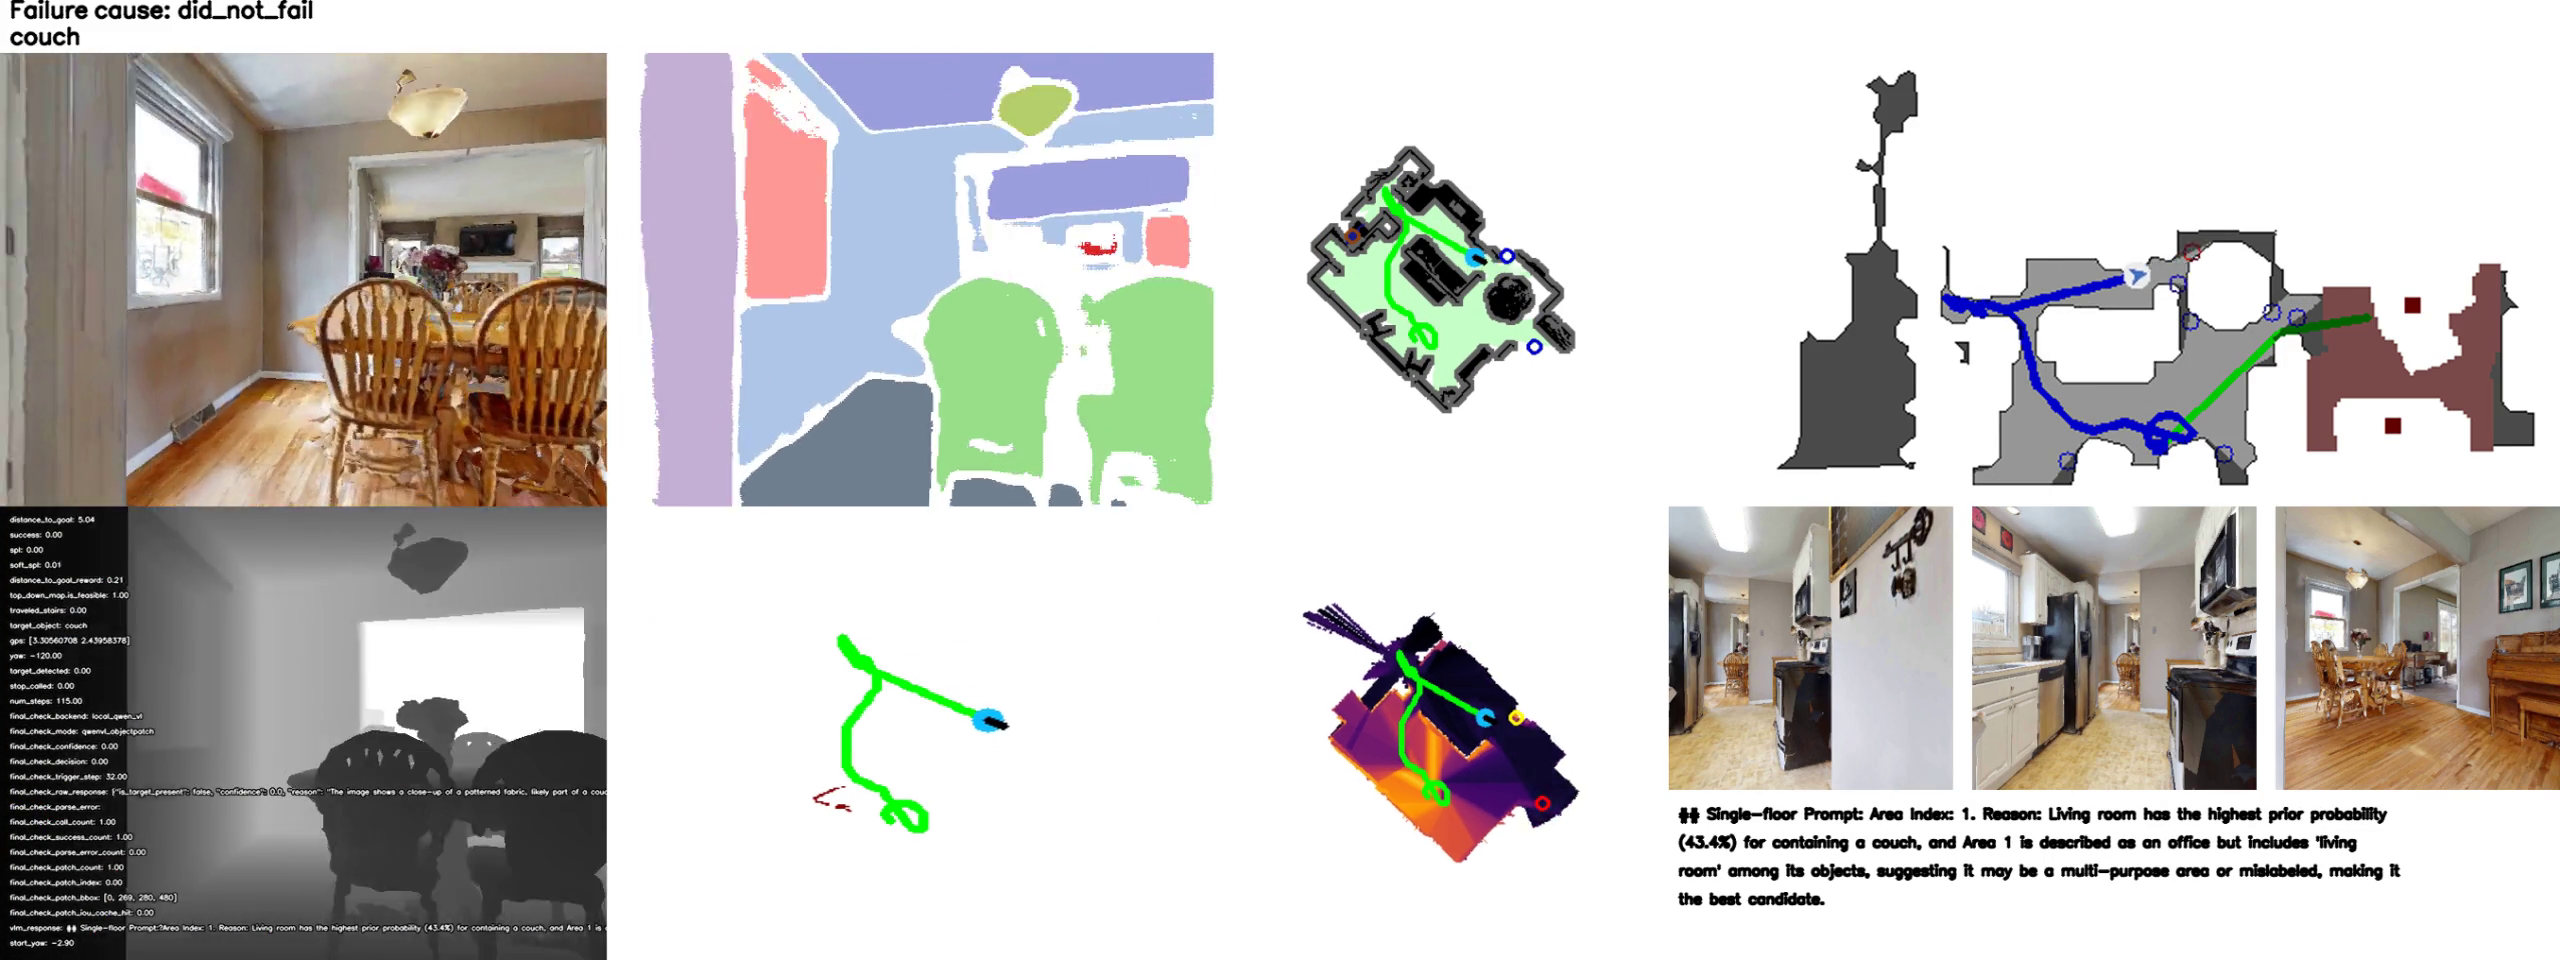
\includegraphics[width=0.45\linewidth]{figures/ascent_selective_success.png} \\
    \small BLIP2 baseline false positive & \small Selective hybrid success
  \end{tabular}
  \caption{Part 3 qualitative example from the fixed demonstration set. The baseline accepts an ambiguous couch candidate and stops incorrectly; the selective hybrid verifier asks for local object-patch evidence and continues until a valid success.}
  \label{fig:qual_part3}
\end{figure}

Figure~\ref{fig:qual_part1} illustrates the Part 1 tradeoff. The Plan A dense-map branch is compact and visually interpretable, and the repaired controller avoids the earlier recovery-loop failure that produced near-zero full-val diagnostics. However, many remaining failures are still stuck or long-horizon exploration failures, so semantic projection alone is not enough. VLFM trajectories are better aligned with exploration, yet false positives remain a frequent failure mode. Figure~\ref{fig:qual_part3} shows why we focus on the final stop gate in Part 3: the most stable improvement opportunity is not global planning, but refusing visually plausible distractors.

\subsection{Part 1 Behavior}
The Plan A visualizations are useful because they expose where the dense-map approach succeeds and breaks. They show that semantic evidence can be projected into a top-down frame, and after the recovery fix the wrapper can use that evidence on a substantial subset of episodes. The remaining failures still concentrate around stuck recovery, noisy semantic peaks, and long exploration. In contrast, VLFM frames show longer exploration, more meaningful frontier movement, and a larger chance of reaching a room that contains the target.

\subsection{Part 3 Behavior}
The ASCENT qualitative pair in Figure~\ref{fig:qual_part3} is representative of the verifier's intended role. The baseline already reaches a semantically plausible region; the mistake occurs at the final confirmation boundary. The selective hybrid does not need to redesign mapping or global planning. It only needs to reject an ambiguous local object patch, continue exploration, and preserve the possibility of a later correct stop. This kind of correction is small in aggregate metrics but highly interpretable.

There are also cases where the verifier hurts. If the target is partially occluded, small, or poorly segmented, the object patch may remove context that a human or BLIP2 would use. If the target category is visually broad, Qwen-VL can answer conservatively. These cases motivate the tri-state design: an uncertain answer should not be treated the same as a confident rejection.

\section{Discussion}
\subsection{What Actually Improved}
The strongest result of the project is not that a larger VLM automatically wins. The evidence points to a more specific conclusion: the stop decision is a high-leverage boundary in zero-shot ObjectNav, and local object-patch verification can improve that boundary when used selectively. In the fixed-200 comparison, the gain is small in absolute SR but clean in interpretation. The selective hybrid reduces false-positive stops while leaving the ASCENT exploration backbone unchanged. This makes the improvement easier to trust than a large aggregate change produced by multiple simultaneous modifications.

The negative results are also useful. The initial dense-map diagnostic branch shows how a small control-state bug can dominate a semantic method, while the repaired Plan A subset shows that fixing recovery restores nontrivial navigation without changing the pretrained visual prior. Naive multi-agent ASCENT shows that adding agents without coordination can reduce performance. Full-frame Qwen-VL shows that a stronger visual-language model can still be distracted by background context. These outcomes motivate the final design: preserve the search policy that already works, and spend extra model capacity only on ambiguous local verification.

\subsection{Metric Interpretation}
SR, SPL, DTG, and failure buckets tell different parts of the story. SR is the headline result, but it hides whether a method succeeds by taking longer paths, rejecting targets, or stopping incorrectly. SPL exposes path inefficiency, while DTG helps distinguish near misses from complete exploration failures. The false-positive and never-saw buckets are especially important for Part 3 because they move in opposite directions: stricter verification can reduce false positives while increasing never-saw outcomes. For this reason, we treat the fixed-200 gain as a controlled improvement rather than a solved navigation system.

\subsection{Next Steps}
The most direct next step is to make verifier invocation adaptive to episode progress. Early in an episode, rejecting a weak candidate is cheap because many frontiers remain. Late in an episode, the same rejection may be costly because the agent has limited time to recover. A better policy could use remaining step budget, frontier count, and repeated candidate history to decide whether an uncertain verifier answer should trigger more local inspection or immediate exploration elsewhere. A second extension is to cache object-patch decisions across viewpoints so that the agent does not repeatedly ask Qwen-VL about the same rejected proposal.

\section{Limitations and Conclusion}
This project has three limitations. First, not all comparisons are on the same episode split; 8/20-episode ablations diagnose behavior, while 1000-episode and fixed-200 runs support stronger conclusions. Second, Qwen-VL object-patch verification requires additional compute and can be over-conservative. Third, exploration, stairs, and local PointNav recovery remain major bottlenecks that a final verifier cannot solve.

The current report also inherits practical limitations from the accompanying results folder. We preserve logs, summaries, selected videos, and derived stills, but not full raw datasets or all debug videos. This is enough to support the written claims, yet a fully independent rerun would still require access to the original simulator assets, model weights, and remote environment configuration.

We conclude that zero-shot ObjectNav improves most reliably when stronger visual-language reasoning is inserted at the right decision boundary. Dense semantic maps establish the basic semantic prior, VLFM frontier scoring makes exploration practical, and ASCENT-style LLM planning handles richer scene structure. The final selective Qwen-VL verifier is not a universal replacement for navigation logic, but it is a useful targeted module: it reduces false-positive stops and gives a small but reproducible fixed-subset SR improvement while preserving the efficient ASCENT backbone.

\clearpage
{\small
\bibliographystyle{ieeetr}
\bibliography{refs}
}

\end{document}
